\chapter{Access control}
\label{ch:ac}
When considering the security requirements of most distributed applications, authorization often emerges as a central element in the design of the whole security system~\cite{woo1998designing}. Therefore, many security properties are determined by the flexibility, trustworthiness and expressiveness of the authorization scheme. Access control is the mechanism that allows resource owners to define, manage and enforce access policies applicable to each resource~\cite{samarati2001access}. Both concepts are related since access control will usually consider authorizations as the basis to produce access decisions.\\

The shift from centralized to decentralized systems and applications poses new requirements in both authorization and access control systems. In the case of centralized systems, the same entity is responsible for the assignment of attributes or privileges to clients (Authorization) and the evaluation of the access requests to determine whether they must be granted or not (Access Control). All the information required to analyse and evaluate the privileges is stored and managed locally in the same system on which the resources reside.\\

We are interested in applying access control to decentralized systems, where interoperability and data portability are the decisive factors. In this chapter, we will investigate and propose an access control model for the social Semantic Web, which takes into account the dynamic evolution of user relations, and which applies to Linked Data generated by users (e.g. profile data, wall posts, conversations, etc.).\\

This chapter is structured as follows. Section~\ref{sec:ac_relwork} offers an overview of existing access control mechanisms, focusing on those that apply to the Semantic Web. Section~\ref{sec:dracl} introduces the concepts of \textit{contexts} and \textit{social proximity distance}, as metrics for a dynamic access control system specific to social Web applications. Section~\ref{sec:sacs} describes our contribution, a Social Access Control Service, which can adapt to the dynamics of human relationships. Finally, we compile and present a list of conclusions.\\

Before discussing our contributions, we first analyse existing access control mechanisms, focusing on those that apply to decentralized systems.

\section{Related work}
\label{sec:ac_relwork}

The basic concepts upon which an access control model is based determines the flexibility of the model to adapt to different environments and systems. Several access control models have been developed, relying on different schemes and requirements. It is important to realize that most of the existing access control models were developed for closed or centralized (i.e. \textit{silo}) environments.\\

There are currently three generic models for access control, the Discretionary Access Control (DAC), the Mandatory Access Control (MAC) and the Role-based Access Control (RBAC). We will briefly cover them below, since they serve as a basis for most access control schemes.

\subsection{Generic access control models}
Discretionary Access Control (DAC) was designed for multi-user databases and systems with a few, previously known, users. Changes were rare and all resources were under control of a single entity. Access was controlled based on the identity of the requester and on access rules stating what requesters are (or are not) allowed to do~\cite{lampson1974protection}.\\

\textbf{Mandatory Access Control} (MAC) had its origins in military environments where the number of users can be quite high, but with a static, linearly hierarchical classification of these users. The model is based on the definition of a series of security levels and the assignment of levels to resources and users. MAC policies control access based on mandated regulations determined by a central authority~\cite{qian1996mac}.\\

\textbf{Role-based Access Control} (RBAC) gets inspiration from the business world. The development of RBAC coincides with the advent of corporate intranets. Corporations are usually hierarchically structured and access permissions depend on the position of the user in the hierarchy, i.e. the role played by the user. RBAC policies control access depending on the roles that users play within the system and on rules stating what accesses are allowed to users in given roles~\cite{ferraiolo2001proposed}.\\

Among the previous models, RBAC is commonly considered a mature and flexible technology. Consequently, it is the most popular mechanism in use today. The main problem with role based access control is that the mechanisms are built on three predefined concepts: \textit{user}, \textit{role} and \textit{group}. The definition of roles and user grouping facilitates management, especially in corporate information systems, since roles and groups fit naturally in the organizational structures of companies. However, when applied to some new and more general access control scenarios (like the social Semantic Web), these concepts are becoming difficult to follow. Furthermore, while static grouping of users of RBAC may suffice in corporate systems, it is not flexible enough to cope with the requirements of more dynamic environments where the structure of groups cannot be foreseen by the administrators of the access control system.\\

Recent technologies such as the Semantic Web increase the complexity and the dependencies of Web services with respect to access control~\cite{sohr2008analyzing}. The adaptation of RBAC to new technologies has been a common starting point. As a result, access control frameworks have been evolving from OASIS XACML (eXtensible Access Control Markup Language)~\cite{standard2010extensible} or X-RBAC~\cite{joshi2004access} which were based on XML to describe the access rights. Unfortunately they did not support a machine interpretation language, which the Semantic Web offers. Furthermore, O-RBAC~\cite{wu2006ontology} adapts RBAC to semantic web technologies by exporting its domain to an ontology specification.

\subsection{Semantic access control mechanisms}
\label{subsec:sem_acl}
The main reason we have decided to analyse access control mechanisms that are based on the Semantic Web and Linked Data principles, is the fact that we are interested in a solution that applies to decentralized Web applications. Moreover, we are also looking for solutions that allow interoperability by easily exporting access control policies along with the user's data. Finally, we are looking for an environment where access to resources is based on reasoning.\\

The ultimate success of a Semantic Web-based access control system, however, will depend as much on the social conditions of its use, as on the underlying technology itself. Much of the power of the Semantic Web lies in its ability to help people share information more richly and to discover subtle information linkages across the Web that are not visible in today's relatively flat online information environment. However, people will not share information freely in an environment that is threatening or antithetical to basic social needs such as privacy, security, the free flow of information, and ability to exercise their intellectual property rights as they choose. Though today's Web falls short in many of these areas, the descriptive and logical functions of the Semantic Web can offer the ability to help people manage their social relationship online, in addition to just managing the traditional information content found on the Web today.\\

\subsubsection{Web Access Control}
Web Access Control (WAC) is a decentralized system in which different users and groups are given various forms of access to resources, and where users and groups are identified by HTTP URIs~\cite{hollenbach2009using}. The system is similar to the access control system used within many file systems except that all etities (i.e. the documents controlled, the users and the groups) are identified by URIs. Agents (groups or users) are identified by the URI of a class of users which, when dereferenced, returns a list of users in the class. This means that a user hosted by an identity platform can be a member of a group hosted by a different Web application or service. Access can be granted for a document on one service to users and groups hosted by other services.\\

The authorization module makes use of a metadata file that contains the access control list (ACL), expressed as Turtle. Metadata is currently stored on a per-directory basis, though the system could easily be modified to store ACL metadata on a per-document basis. The server directs clients to the ACL for a given file using the link \textit{rel=meta} HTTP header~\cite{connolly1999entity}.\\

The ACL ontology used is the Web Access Control Ontology [13]. For a given rule, \textit{acl:accessTo} defines a resource that access is being granted to. \textit{acl:agent} and \textit{acl:agentClass} define an agent or agent class (i.e. any foaf:Person) as being granted access. \textit{acl:mode} defines the set of access modes that are granted to the agent or agent class. Finally, \textit{acl:defaultForNew} optionally defines the default access rules for new (future) documents in a directory.\\

Example~\ref{ex:acl-webacl} displays a simple ACL metadata file. This file grants to the WebID \textit{https://barry.example/profile\#me} Read, Write, and Control access to the file \textit{foaf.rdf}, and Read access to \textit{foaf.rdf} to all authenticated WebID users. It also grants \textit{barry} Read, Write, and Control access by default for new files.\\

\begin{example}[h]
\begin{minted}{turtle}
@prefix acl: <http://www.w3.org/ns/auth/acl#> .
[] a acl:Authorization ;
    acl:defaultForNew <.> ;
    acl:accessTo <foaf.rdf> ;
    acl:agent <https://barry.example/profile#me> ;
    acl:mode acl:Control, acl:Read, acl:Write .
    
[] a acl:Authorization ;
    acl:accessTo <foaf.rdf> ;
    acl:agentClass <http://xmlns.com/foaf/0.1/Agent> ;
    acl:mode acl:Read .
\end{minted}
\caption{A simple ACL metadata file.}
\label{ex:acl-webacl}
\end{example}

The three types of access that can be granted are \textit{Read}, \textit{Write}, and \textit{Control}. The Read and Write modes control access to normal files stored on the server. Control is essentially a special form of Write access. Providing Control access to a file allows a user to edit the ACL metadata for that file. Authorization is determined by running a set of SPARQL queries to decide if the user is granted access either as an agent or as a member of an agent class.\\

If a user attempts to use an HTTP method that they are not permitted to use, they receive an HTTP 403 response from the server. For instance, based on the ACL file presented in Example~\ref{ex:acl-webacl}, if a user authenticated with the URI \textit{http://www.example.com/foaf\#me} tries to delete \textit{foaf.rdf} with an HTTP DELETE request, the server would see that only \textit{barry} has Write access (which also includes the delete operation) and will then respond with \textit{HTTP 403 Forbidden}.\\

However, WAC can only restrict access to files as a whole, not to the specific resources (i.e. triples) located within RDF files (e.g. a user's profile). 

\subsubsection{Accountability in RDF}
Accountability in RDF (AIR)~\cite{kagal2011gasping} is a Semantic Web-based rule language that provides access control while focusing on generating explanations for its inferences and actions as well as conforming to Linked Data principles.\\

AIR is an extension to N3Logic~\cite{berners2008n3logic}, which is a minimal extension to the RDF data model such that the same language can be used for logic and data. AIR has been structured to meet the justification and rule reusability requirements of Web information systems. Along with including the N3Logic features of scoped negation (i.e. the ability for a specific given document or an abstract formula to objectively determine whether or not it holds, or allows one to derive a given fact), scoped contextualized reasoning (i.e. to reason using a first order logic but without classical negation), nested graphs, and built-in functions, AIR is focused on generating useful justifications for all actions made by the reasoner. Like N3Logic, AIR is written in N3~\cite{berners2000primer}, which provides a human-readable syntax for a superset of RDF. N3Logic extends the RDF data model by supporting the quantification of variables as URIs with the \textit{@forAll} and \textit{@forSome} directives. It also permits the inclusion of nested graphs by using curly braces to quote sub-graphs.\\

AIR consists of a set of built-in functions and two independent ontologies -- the first one (Figure~\ref{fig:airr_onto}) is for specifying AIR rules, while the other one is for describing justifications of the inferences made by AIR rules (Figure~\ref{fig:airj_onto}), which help to verify the accuracy and validity of access control policies during audit processes. The built-in functions allow rules to access Web resources, query SPARQL endpoints, and perform scoped contextualized reasoning, as well as basic math, string and cryptographic operations.\\

\begin{figure}[h]
  \begin{center}
    \includegraphics[width=350px]{img/air_ontology.jpg}
        \caption{AIR rule ontology, as presented in \textit{Gasping for AIR Why we need Linked Rules and Justifications on the Semantic Web}~\cite{kagal2011gasping}.}
        \label{fig:airr_onto}
  \end{center}
\end{figure}

AIR also supports \textit{Linked Rules}, which like most rules (e.g. whether laws, security policies, business rules, or workflow plans), are rarely defined by a single entity or exist in a single document. They usually comprise of several interdependent rules that are defined and maintained by different entities. Additionally, rules may reference external rules, including those of other organizations.\\

\begin{figure}[h]
  \begin{center}
    \includegraphics[width=350px]{img/airj_ontology.jpg}
        \caption{The AIR justification ontology, as presented in \textit{Gasping for AIR Why we need Linked Rules and Justifications on the Semantic Web}~\cite{kagal2011gasping}.}
        \label{fig:airj_onto}
  \end{center}
\end{figure}

AIR rules are defined using the following properties: \textit{air:if} , \textit{air:then}, \textit{air:else}, \textit{air:description}, \textit{air:rule} and \textit{air:assert}. Every rule is named with a URI, and rules are grouped into \textit{air:RuleSets} or nested under other rules (Figure~\ref{fig:airr_onto}). This nesting can happen either under the \textit{air:then} property or the \textit{air:else} property. The rules nested directly under the RuleSet are referred to as the top rules of the ruleset. A chain of rules is defined as a sequence of rules, such that every rule, barring the first in the chain, is nested under either the \textit{then} or the \textit{else} of the preceding rule.\\

There are three kinds of rules in AIR -- \textit{air:BeliefRule}, \textit{air:HiddenRule} and \textit{air:ElidedRule}. All rules are, by default, Belief rules. The descriptions and conditions of Belief-rules contribute to the overall justification. :ViewImageRule1 in Example~\ref{ex:air_rule} is an typical rule example of a Belief rule. In contrast, Hidden rules and Elided rules are used to modify the default justification.\\

\begin{example}[h]
\begin{minted}{turtle}
@prefix air: <http://dig.csail.mit.edu/TAMI/2007/amord/air#> .
@forAll :REQUESTER, :PIC .

:ViewImageRule1 a air:BeliefRule;
  air:if { :REQUESTER a req:Requester ;
               req:requestedImg :PIC.
            :PIC sioc:topic
               <http://ann.example/profile#me>.
  };
  air:then [ air:description (
               "If the picture requested contains "
               "Ann, then execute Ann's policy "
               "about image access");
             air:rule ann:MyImgPolicy
  ].
  
ann:MyImgPolicy
  air:then [ air:description(
               "Ann's policy was executed");
             air:assert {
               :REQUESTER req:compliant-with :BarryRuleSet }
  ];
  air:else [ air:assert {
               :REQUESTER req:non-compliant-with :BarryRuleSet }
  ].
\end{minted}
\caption{A typical AIR RuleSet.}
\label{ex:air_rule}
\end{example}

Example~\ref{ex:air_rule} contains an AIR RuleSet, in which Ann has created policy to determine whether access to one of her pictures should be granted. AIR uses N3Logic syntax to declare variables. In this example, @forAll is used to declare two universal (i.e. global) variables, \textit{:REQUESTER} containing the requester and \textit{:PIC}, which contains the URI of the resource in question (i.e. the picture).\\

Next, we define a rule called \textit{:ViewImageRule1}, of type \textit{air:BeliefRule}, which contains the logic we want to apply for our policy. In this case we have a typical if $\rightarrow$ else logic, stating that if a :REQUESTER is trying to request access to :PIC and the picture contains Ann's WebID, then the rule should apply the policy \textit{ann:MyImgPolicy}, which is defined below.\\

\textit{ann:MyImgPolicy} extends the logic flow by supplying additional actions. Here, it uses the \textit{air:assert} verb to verify that the :REQUESTER is compliant with the rule set she created for this picture, and which is called \textit{:BarryRuleSet}. The resource \textit{:BarryRuleSet} contains a list of rules which involve Barry. AIR semantics will cause them to be included during the reasoning of their parent rule, \textit{:ViewImageRule1}. An \textit{air:else} fall-back case can be created, in order to apply a different action if the :REQUESTER is non-compliant with the current policy.


\subsubsection{Social Semantic Web Access Control}
Social Semantic Web Access Control~\cite{villata2011social} is based on the \textit{Social Semantic SPARQL Security for Access Control} vocabulary -- S4AC (cf. Figure~\ref{fig:s4ac_onto}), a lightweight ontology that allows users to specify fine-grained access control policies for their RDF data -- e.g. restrict the access to resources within RDF documents.\\

S4AC allows the data provider to specify the access privilege he wants to grant -- i.e. \textit{Read}, \textit{Update}, \textit{Create}, and \textit{Delete}. The main component of the vocabulary is the \textit{Access Condition} which is a SPARQL 1.1. ASK clause that specifies the condition to be satisfied in order to grant the access, which can be evaluated either conjunctively (conditions composed of one or more atomic value constraints linked by \textit{logical-and} operators) or disjunctively (where conditions consist of one or more conjunctive constraints linked by \textit{logical-or} operators). Data providers can define Access Policies, where the set of Access Conditions is applied only to the data concerning a specific subject (using the property dcterms:subject), and the Access Conditions can be bound to specific values to provide an \textit{Access Evaluation Context}. A graphical representation of the S4AC vocabulary can be found in Figure~\ref{fig:s4ac_onto}.\\

\begin{figure}[h]
  \begin{center}
    \includegraphics[width=350px]{img/s4ac_ontology.png}
        \caption{The S4AC ontology. Dashed lines and contours are used to represent external classes, properties and relations.}
        \label{fig:s4ac_onto}
  \end{center}
\end{figure}

The Access Condition (AC) grants or restricts the access to the data. If the ASK query returns true, access is granted to the user. In order to return to the user a more informative answer if the access is denied, the authors have introduced the property \textit{:hasCategoryLabel}. This property allows to associate to each AC one or more natural language labels that "identify" the access condition. The label can be included in the response that is returned to the user to provide him/her the reasons of the denial.\\

The Access Evaluation Context (AEC) is represented in the ontology as the class \textit{AccessEvaluationContext} which has two properties, \textit{:hasVariable} and \textit{:hasValue}, which are respectively the variable, and the value to which the variable is bound. AEC is used
to provide a standard evaluation context to the access conditions (e.g. the requesting user and the resource provider).\\

A very interesting feature is the \textit{Access Tagging Rule} (ATR), which is used to declare that the access conditions in the AC set applies to any RDF graph tagged with one or more tags from a set of tags. In other words, users can simply "tag" certain resources with a specific tag name, for which an AC has been previously specified.

\subsubsection{SHI3LD}
Shi3ld~\cite{costabello2012shi3ld} is an access control framework for querying Web of Data servers. It protects RDF stores from incoming SPARQL queries, whose scope is restricted to triples included in accessible named graphs only~\cite{carroll2005named}. In particular, Shi3ld determines the list of accessible graphs by evaluating pre-defined access policies against client attributes sent with the query.\\

The Shi3ld policy manager allows the definition of context-aware access conditions featuring user, environment (time and location above all), and device attributes. Moreover, such application allows a simpler definition of new named graphs over a set of existing triples.\\

Shi3ld adopts exclusively Semantic Web languages, reuses existing proposals, and protects data up to triple level. The model is grounded on two ontologies: \textit{S4AC}\footnote{http://ns.inria.fr/s4ac/v2/s4ac\_v2.html} (cf. Figure~\ref{fig:s4ac_onto}) deals with core access control concepts and \textit{PRISSMA}\footnote{http://ns.inria.fr/prissma/v1/prissma\_v1.html} focuses on the mobile context.\\

The main component of the S4AC model is the Access Policy which defines the constraints that must be satisfied to access a given named graph or a set of named graphs. If the Access Policy is \textit{satisfied}, the data consumer is allowed to access the data. Otherwise, access is denied. The constraints specified by the Access Policies concern the data consumer, the device, the environment, or any given combination of these dimensions. Access Conditions are expressed as SPARQL ASK queries. Each Access Policy is associated to an Access
Evaluation Context, an explicit link between the policy and the actual context data used to evaluate the Access Policy.\\

The Shi3ld framework also adopts \textit{PRISSMA}, a vocabulary providing classes and properties that serve to model core mobile context concepts, but is not meant to deliver yet another mobile contextual model. Instead, well-known Web of Data vocabularies and recent W3C recommendations are reused. The mobile context is seen as an encompassing term, an information space defined as the sum of three different dimensions: the mobile \textit{User} model, the \textit{Device} features and the \textit{Environment} in which the action is performed.\\

\subsection{Synthesis}
In this section, we have presented recent work that applies to access control for Semantic Web resources. We have selected several solutions that deal with access control in a decentralized environment.\\

The first solution is called \textit{Web Access Control} (WAC), and it resembles to the typical access control of a file system, in which users and groups (identified by URIs) are given read and write access to documents. To describe access control policies, WAC uses it's own ontology, called the \textit{Web Access Control Ontology}. An important drawback of WAC is that it only restricts access to files as a whole, not to the specific resources (i.e. triples) in an RDF document (e.g. a user's profile). Web Access Control ontology was published by the W3C, and the its application process will soon begin standardization within the W3C.\\

The second one is called \textit{Accountability in RDF} (AIR), which is a Semantic Web-based rule language that provides access control while focusing on generating explanations for its inferences and actions, so that rules can be verified during a policy audit. AIR consists of a set of built-in functions and two independent ontologies, one for specifying AIR rules and the other one for describing justifications of the reasoning performed using AIR rules. As opposed to WAC, AIR can be applied to documents as well as to resources within RDF documents.\\

The third solution, the \textit{Social Semantic Web Access Control} (SSWAC) allows users to specify fine-grained access control policies for their RDF data, in order to restrict or allow access to resources within RDF documents. SSWAC uses the \textit{Social Semantic SPARQL Security for Access Control} vocabulary to define its access control policies. Compared to the previous access control solutions, SSWAC uses the concept of \textit{tags}, to assign specific labels to resources. This feature is particularly relevant to us, as you will be able to see in the following section.\\

Finally, Shi3ld offers a context-aware access control framework for consuming the Web of Data from mobile devices. The drawback of such framework is that it relies on the assumption that dataset administrators have a proficient knowledge of RDF and SPARQL, and that they are able to manage vocabularies and define new named graphs.\\

Unfortunately, defining a set of static policies may not equally apply in every situation. Additionally, static policies do not take into consideration the dynamics of human relationships and the pace with which they evolve. Furthermore, most semantic access control systems apply to resources in the form of documents, often not being able to apply to the triples level.\\

In the following section, we propose a context-aware access control service, which provides static access control systems with means to manage the constant and dynamic evolution of user relationships. 

\section{Proposed social metrics for access control}
\label{sec:dracl}
A major drawback of existing Access Control mechanisms is that in most cases they are difficult to maintain and they apply to documents. In the case of social Web applications, creating access control policies that accurately reflect the user's privacy expectations is often difficult if not outright impossible~\cite{madden2012privacy}. In general, privacy is difficult to measure, especially since it's hard even for the users themselves to quantify. For example, photos alone are likely to have wildly varying privacy requirements, depending on who is in the photo, where it was taken, what the audience is, etc. More worryingly, even for photos for which the privacy settings have been modified by the user, the modified settings usually match users expectations less than 40\% of the time~\cite{liu2011analyzing}.\\

We believe that current access control mechanisms suffer from a lack of \textit{context}, specific to relationships between people. We borrow the use of the terms \textit{context} and \textit{situation} in order to redefine what context is, based on a definition first provided by Dey~\cite{dey2001understanding}:
\begin{quote}``Context is any information that can be used to characterize the situation of an entity, with respect to the relationship towards one or multiple other entities.''\end{quote}

We consider that depending on different contexts and situations, access to resources can be handled differently~\cite{sambra2012context}. Additionally, we would like to propose a social distance metric called \textit{proximity}, which also plays a very important role in our model. We shall now take a detailed look at both context and proximity, as metrics for a dynamic access control system tailored for social Web applications.

\subsection{Contexts expressed as labels}
The computer representation of groups usually describes an organization of users of a specific software product or feature, considered together because of the similarities they share. However, once we try to directly apply this notion to the social Web, we have to face the fact that people are unique individuals. We can always try to divide groups into sub-groups, but we must keep in mind that our social relations can be very dynamic and therefore difficult to manage in an electronic environment.\\

On the other hand, we are capable of differentiating between a large number of social contexts, often with very subtle differences. To help us do this, we label people and objects, and as our relation towards them evolves over the time, we either preserve or modify the labels. As opposed to grouping people, one or more labels can be dynamically assigned to people and data, and can also be instantly created when the need arises, similar to how tags or keywords are created on blogging platforms (e.g. \verb+#beachparty2013+, \verb+#soccerteam+, \verb+#family+, etc.). We have therefore decided to apply the concept of \textit{contexts} expressed through \textit{labels} in our proposed model.\\

\subsection{Social proximity distance}
Current social Web applications are usually limited in the types of relations they express (\textit{friends} on Facebook, \textit{circles} on Google+ or \textit{aspects} on Diaspora), and they often do it in a very minimal way, without the means to express strength for relations. For example, we are familiar with relations between people (e.g. "Ann knows Barry" or "Ann just became friends with Barry") and relations between people and objects (e.g. "Ann owns this image" or "Ann shared this file").\\

A typical social web application will describe the relation between Ann and Barry as a statement that Barry is included among Ann's \textit{known} people. Finding the right terminology is very important in this case, since for some people it implies the fact that Ann is \textit{friends} with Barry, while in fact it only describes a unidirectional relationship between Ann and Barry. Current popular social networks consider that Ann "is friends" with Barry if and only if the reciprocal is also true, meaning Barry "is friends" with Ann. Additionally, they do not offer the possibility to convey what kind of relationship it is, since they lack a semantic description of said relationship. At the same time, it is important to preserve the privacy aspects of disclosing relation types (e.g. Ann may not want Barry to know that he was labelled as a "bad co-worker").\\

\begin{figure}[h]
  \begin{center}
    \includegraphics[width=270px]{img/proximity.pdf}
        \caption{Our representation of contextualized proximity levels, based on Hall's concept of personal spaces.}
        \label{fig:proximity}
  \end{center}
\end{figure}

In The Hidden Dimension~\cite{edward1966hall}, Hall examines the various cultural concepts of space between people and how differences among them affect modern society. Hall talks about four spaces: \textit{intimate}, \textit{personal} (which we have renamed to \textit{close}), \textit{social} and \textit{public}. Applying these concepts to a social platform helps define the weight of relationships. From now on, we will refer to this metric as \textit{proximity} (not related to physical or geographical proximity).\\

In the scope of the service we will propose in the following section, access control applies to relations between users and resources. Resources can either be RDF triples generated by the user (e.g. personal profile information, comments, etc.) or non-RDF files (e.g. images, videos, documents, etc.). We will only focus on the RDF type, since numerous access control mechanisms already exist for ordinary files.\\

To describe relationships between users, we start with the root class called \verb+Relationship+, which corresponds to the public space and by itself implying an unspecified relationship. Next we have four subclasses, \verb+Public+, \verb+Social+, \verb+Close+ (corresponding to the Personal level), and \verb+Intimate+, all corresponding to a proximity level described by Hall~\cite{edward1966hall}. However, these relationship types do not provide context. To convey context, labels (i.e. \verb+#siblings+, \verb+#sportsteam+) can be assigned to each subclass (Figure~\ref{fig:proximity}).\\

\section{Proposed Social Access Control Service}
\label{sec:sacs}
Our proposed solution, the \textit{Social Access Control Service} (SACS) is orthogonal to existing access control systems, as it is based on social proximity levels and labels together with our online interactions (e.g. sharing a resource with someone, tagging a user within a specific context, etc.), in order to apply access control policies to a user's online social resources (e.g. a user's profile, wall posts, conversations).\\

SACS is comprised of two distinct sub-services, a \textit{Relationship Monitor} (RM) engine and a \textit{Static Access Control} (SAC) engine, as seen in Figure~\ref{fig:acs_architecture}.\\

\begin{figure}[h]
  \begin{center}
    \includegraphics[width=250px]{img/reasoning_engine_diagram.pdf}
        \caption{Architecture of our social access control service.}
        \label{fig:acs_architecture}
  \end{center}
\end{figure}

The RM engine handles the dynamic evolution of user relationships and it applies to user generated content (e.g. profile information, wall posts, conversations, etc.). It relies on a Relationship History database when suggesting access control policies or taking decisions (Section~\ref{subsec:rme}). This database contains a list of interactions between the user and his/her friends. History entries are independently created whenever the user interacts with other people, such as sharing a resource with someone, tagging a person within a specific context, etc.. As this system is designed to run on a device controlled by the user, the privacy implications resulting from such a collection of social interactions should be reduced.\\

A different component, the SAC engine, is used to define static access control policies that apply to most types of resources (either RDF or binary documents). For policy enforcing, the SAC may rely on either WAC or AIR (cf. Figure~\ref{fig:acs_architecture}), which would then store access control rules in the policy database, to facilitate access control management. Rules are represented using RDF, which means that they can be easily exported to be used on other platforms. The SAC engine can operate independently from the RM engine, as you will see in Section~\ref{subsec:acs}.\\

Next, before going into detail for each component of the architecture, we propose a short motivating example to put into perspective the advantages of a dynamic social access control service.

\subsection{Motivating example} 
\label{subsec:example}
After having met Ann, Barry decides to add her as a "known person". The system defines the initial weight of the link between Barry and Ann to be \textit{half}, since this relationship can be mutual (full). Based on the current weight, the default corresponding proximity level for Ann is \textit{Public} (Fig.~\ref{fig:proximity}). If Ann also decides to include Barry as a known person, then the weight of the link becomes \textit{full}, corresponding to the \textit{Social} proximity level. At this point, if Barry does not provide any context information for the relation between him and Ann, the system assigns the label \verb+#acquaintances+ based on the default value corresponding to the \textit{Social} proximity level for Friends (Fig.~\ref{fig:proximity}).\\

Next, depending on how often Barry communicates with Ann, either directly or by including Ann in specific contexts (i.e. \verb+#beachparty+), the proximity level may change. For example, after attaining a certain threshold triggered by the transition from \textit{Social} to \textit{Close} proximity levels, content labelled with \verb+#closefriends+ may become available for Ann (Figure~\ref{fig:proximity}). On the other hand, the lack of interaction during a long period of time may decrease the proximity level, resulting in creating distance between them. In other words, the RM considers that Ann no longer belongs to the same proximity level, and can even modify one or more of Ann's labels if so configured. In this case, special alerts can be displayed if Barry decides to share content (specific to the \textit{Personal} level) with Ann after her proximity level has decreased, going from \textit{Personal} to \textit{Social}, or it can automatically remove Ann from the list of recipients.\\

Let us now investigate the components of our Social Access Control Service and the way they influence access control decisions, beginning with the Static Access Control engine.

\subsection{The Static Access Control engine}
\label{subsec:acs}
As the name suggests, the \textit{Static Access Control} engine handles predefined privacy rules. Even though it is an important component of SACS, it does not require the RM engine to be present and functioning. However, in this case, users will have to manually define access control policies for their data. The SAC engine has been implemented as a feature of MyProfile (see Section~\ref{sec:sac_implem} of Chapter~\ref{ch:implementations}).\\

Please note from Figure~\ref{fig:acs_architecture} that the SAC engine contains two modules, the \textit{Contexts} module which is our contribution and will be presented next, and the generic module which can be based on a static semantic access control mechanism like WAC or AIR. The generic module will not be presented as it is out of scope for this thesis. However, the purpose of the generic module is to provide an additional layer of access control for documents, and depending on the user's preferences it may or may not be enabled on the system.

\subsubsection{Contexts module}
Building on the examples provided above and also considering the fact that users do not enjoy spending time managing privacy rules, we can imagine a set of default rules, specific to each proximity level. Defining a policy in our proposed solution involves first creating a context (label). Resources as well as users are matched to specific contexts. If a match is found between the context that is bound to the resource and the context assigned to the user, then the user will be granted access to the resource.\\

The relationship between a context and a resource or a user is defined in a graph in form of triples, following the basic principles of Linked Data. Contexts can be assigned to all resources at the triple level. For each particular user of the system, the system assigns a graph called \textit{contexts}, which is a collection of contexts created by the user (Figure~\ref{fig:context_context}), and also assigns graphs for each context (Figure~\ref{fig:context_tags}). All context graphs are be stored in the \textit{Policies Database}.\\

\begin{figure}[h]
  \begin{center}
    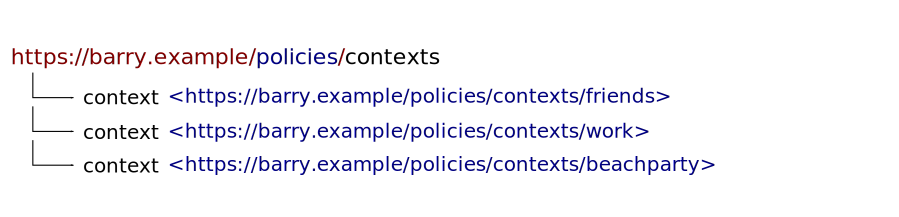
\includegraphics[width=270px]{img/context_tags.pdf}
        \caption{Graph containing all contexts defined by Barry.}
        \label{fig:context_tags}
  \end{center}
\end{figure}

Each context is defined as a resource graph with its own unique URI. To give a context a clear meaning, each defined context has a name and an optional description field (Figure~\ref{fig:context_context}). Since the context's primary function is to define the relationship between a user and a resource, one context can be bound to several resources and users (Figure~\ref{fig:context_context}). For instance, a context graph may contain profile data (e.g. phone numbers, full name, homepages, etc.), wall posts, or even conversations between users (in the form of SIOC\footnote{http://rdfs.org/sioc/spec/} resources).\\

However, since there is no such concept as "pointers" (like the ones found in C/C++), this operation implies that each time a context is assigned to a resource, the resource URI (or literal value) will be copied into the context graph. Another significant drawback resulting from the lack of pointers is that updating a resource in the user's profile must be reflected in all context graphs containing that particular resource.\\

\begin{figure}[h]
  \begin{center}
    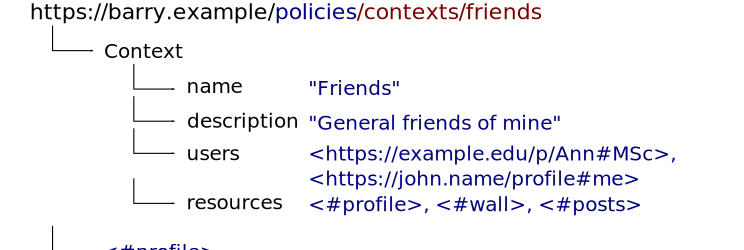
\includegraphics[width=240px]{img/context_context.pdf}
        \caption{Example of a graph for the context \textit{\#friends}}
        \label{fig:context_context}
  \end{center}
\end{figure}

For example, let's consider that Barry assigns the \verb+#friends+ context to his phone number, thus limiting access to this resource. In case this particular context does not exist, the system creates a new context graph, with the URI \textit{https://barry.example/policies/contexts/friends} (Figure~\ref{fig:context_context}). Since the phone number is part of the user profile, the system creates a pointed graph called \textit{<\#profile>} in which it copies the phone number entry. Next, Barry wants to allow Ann to view his phone number. To do this, he has to assign the same context label (i.e. \verb+#friends+) to the user Ann, which is identified by her WebID. The system will now add Ann's WebID to the list of users to which the context \verb+#friends+ has been assigned to (Figure~\ref{fig:context_context}).\\

Several contexts can be assigned to a resource or to a user. Users in the same proximity level can have different contexts, corresponding to different resources, and each user can only see the resources assigned to them. It should be noted that if the user has no defined access control policies, then all the resources they own are publicly available by default.\\

Let us now take a look at the algorithm that is applied in order to match users and resources to contexts, each time a request is received by the system.


\subsubsection{Context matching algorithm}
\label{subsec:context_algo}
Figure~\ref{fig:context_matching} presents a simple algorithm, describing the process of context matching. The goal of this process is to finally return a \textit{unique view} of requested resources (e.g. a user's profile, a wall, a conversation, etc.), based on their corresponding level of access.\\

\begin{figure}[h]
  \begin{center}
    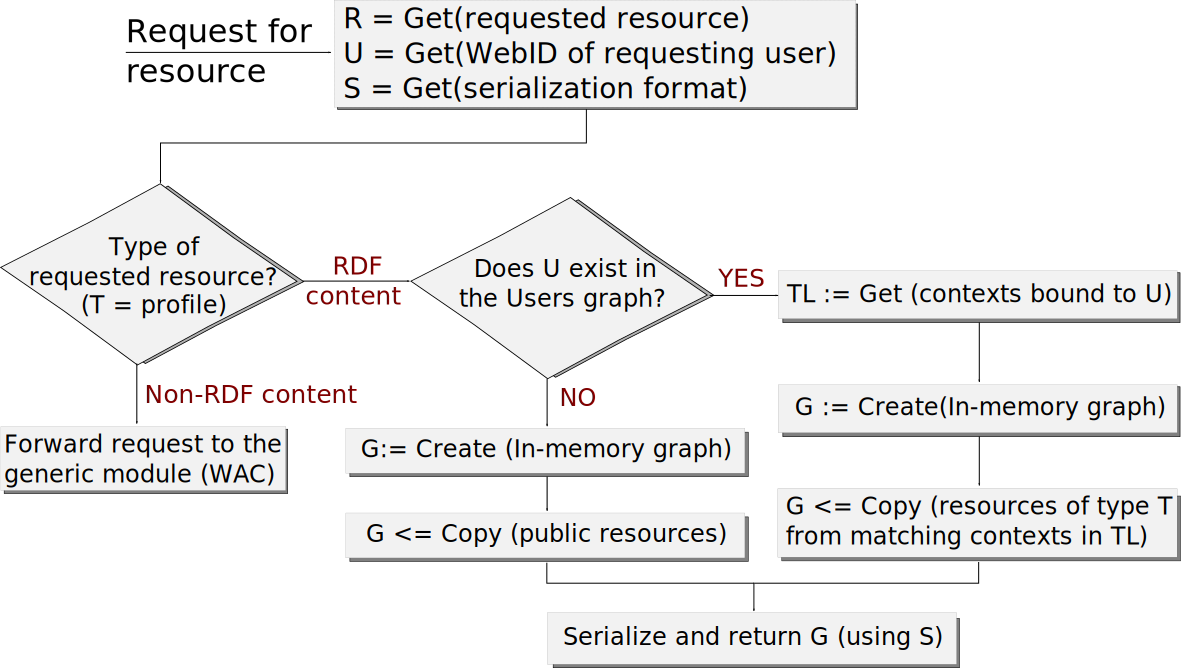
\includegraphics[width=270px]{img/algorithm-matching.pdf}
        \caption{Context matching algorithm.}
        \label{fig:context_matching}
  \end{center}
\end{figure}

The information contained in the \textit{Request} includes the type of the requested resource (T), the WebID of the requester (U) and the data serialization format (S) for the response (e.g. Turtle, RDF/XML, N3, etc.). At this point, we assume that the requesting user has already been authenticated at the moment of the request. If the user has not been authenticated, only the public view of the requested resource is returned.\\

The following step of the algorithm is to lookup the requester in the graph of users belonging to the resource owner. If there is no match, the requester receives only the public view of the requested resource. Otherwise, all contexts assigned to the requester's WebID are extracted, and a list of all contexts URIs (TL) is created.\\

The next step is to create a temporary, in-memory graph (G), to store only the resources matching the requester's access policies. This graph will only be used during the processing of the algorithm, to hold the contents of the reply.\\

Once the graph has been created, it is time to copy all resources belonging to the list of contexts (TL), and which correspond to the type of the request (e.g. a profile, a wall, a conversation, etc.).\\

Finally, the graph (G) is serialized in the requested format (S) before being returned to the requesting user (U). As soon as the contents of (G) have been sent through HTTP(S), the graph is destroyed and memory is freed.


\subsection{The Relationship Monitor engine}
\label{subsec:rme}
The \textit{Relationship Monitor} engine (RM) is tasked to analyse the dynamicity of relationships between two given users, in order to either provide notifications for potential privacy issues that may arise when disclosing information, or it may even modify existing access control policies for incoming requests (if so configured).\\

The RM applies to two distinct types of actions. First, for assigning context labels when disclosing information, and second for handling a request for a resource.

\subsubsection{Assigning context labels}
When a user intends to limit the audience for some of his/her private information (e.g. religious views, sexual orientation, etc.), he/she can assign one or more context labels to the information that is to be protected, as well as to the audience in order to indicate who can access the information.\\
	
During this labelling process, the RM analyses user interaction data from the Relationship History database (Figure~\ref{fig:acs_architecture}), corresponding to the selected audience. Typical examples of user interactions include sharing a picture within a specific context (i.e. \verb+#closefriends+), explicitly changing a user's proximity level, excluding a user from a given context (without permanently removing him/her) when sharing a resource, the number of times users exchange messages (as a function of time), etc.\\

We can imagine that during a user's online activity, several interactions are considered pertinent by the RM. The user should always be allowed to select which types of interactions he/she considers pertinent, or potentially be allowed to create new interaction types. However, since we have not yet implemented the RM in a real application, we will restrict ourselves to proposing several types as follows:

\begin{enumerate}
\item Explicitly sharing a resource (i.e. photo, video, file) with a user.
\item Explicitly sharing profile information (i.e. phone number, email address, etc.) with a user.
\item Assigning a context label to a user, and implicitly a proximity level, since contexts are bound to one or more proximity levels.
\item Removing a context label from a user.
\item Assigning a proximity level to a user.
\item Modifying the proximity level for a user, either manually or by assigning/removing context labels.
\end{enumerate}

Based on the interactions in Relationship History database, the RM may alert the user (i.e. provide visual indications) to a possible change in their relationship. For instance, a warning message may appear if the resource owner is in the process of assigning a context label (which corresponds to a specific proximity level) to a user which is in a more distant proximity level.

\subsubsection{Handling requests}
When requests are received, they are first processed by the RM in order to be classified into two major categories, based on the relationship between the requesting user and the owner of the requested resource (Figure~\ref{fig:algorithm_rme}).\\

In the first category, no predefined privacy policy exists for the requesting user, and the requesting user is not related to the resource owner or any of the resource owner's known people. This is typically the case of an unknown user or a user that is not authenticated. At this point, the RM forwards the request directly to the SAC, where predefined privacy policies are applied for the resource in question.\\

In the second category, the requesting user already has a relationship with the resource owner or with one of his/her known people, based on the authentication credentials it provides alongside the request. In this case, two additional sub-categories exist, and the request is handled by the RM according to the type of the proximity distance and contexts between the requesting user and the resource owner.\\

The first sub-category applies to the cases where a less dynamic relationship exists between the requesting user and the owner of the resource. Please note that through configuration options which are out of scope for the algorithm presented in Figure~\ref{fig:algorithm_rme}, resource owners have the possibility to deliberately disable the RM for relationships they consider less likely to be susceptible to dynamic changes. For example, people labelled as \verb+#family+ or \verb+#girlfriend+. By default, the RM is disabled for users belonging to the \textit{intimate} proximity level.\\

The second sub-category applies to all requesting users that have a dynamic relationship with the resource owner. A history of all interactions between the requesting user and the resource owner is kept in the \textit{Relationship History} database (Fig.~\ref{fig:acs_architecture}).\\

The RM decides whether or not to allow access to resources, based on existing privacy policies defined by the SAC engine, as well as based on data from the Relationship History database corresponding to the relationship between the requesting user and the resource owner. If so configured, the RM can potentially add, update or remove existing rules within the SAC or theoretically, on local and/or remote access control systems like the ones presented in Section~\ref{subsec:sem_acl}. The RM may also support an \textit{unsupervised operation mode}, though this is considered as future work. The unsupervised operation mode would normally involve taking access control decisions based on decision factors resulted from machine learning or the user's decision history, without awaiting user input. However, unless properly configured, the unsupervised operation mode may provide unwanted results and should be activated upon explicit request from the user. Additionally, the RM may be disabled at any time, leaving the SAC in charge of handling all access control.\\

Currently, two metrics are utilized during RM's decision making process. They are the \textit{proximity distance} and the \textit{contexts}. Next, we will go through a typical decision making process for our protagonists, Ann and Barry.

\subsubsection{RM's decision making process}
Before beginning, we would like to mention that the user's social interactions can only be monitored if the RM is part of the social Web application.\\

The algorithm behind the RM's decision making process can be seen in Figure~\ref{fig:algorithm_rme}.\\

\begin{figure}[h]
  \begin{center}
    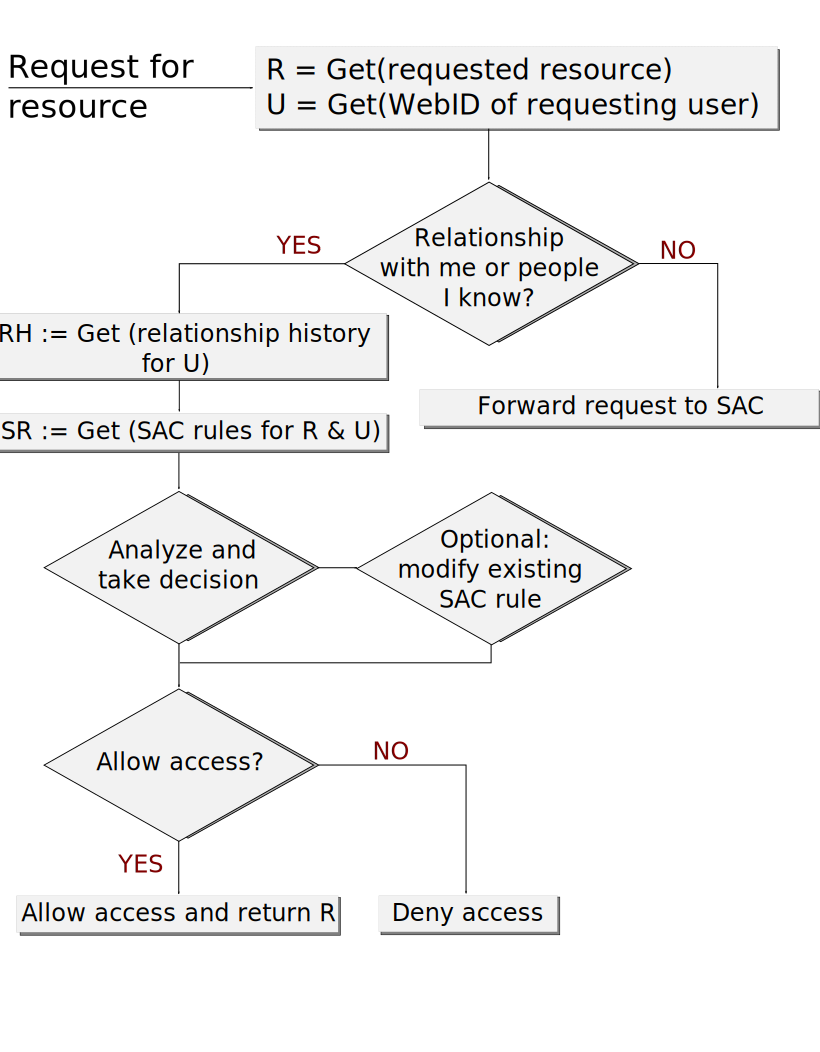
\includegraphics[width=270px]{img/algorithm-rme.pdf}
        \caption{RM's decision making process.}
        \label{fig:algorithm_rme}
  \end{center}
\end{figure}

The information contained in the \textit{Request} includes the requested resource (R) and the WebID of the requester (U). At this point, we also assume that the requesting user has already been authenticated at the moment of the request. If the user has not been authenticated, the process will consider the user to be \textit{undetermined} (i.e. anyone with public access).\\

The following step is to decide if the user in question has any relationships with the resource owner or people known by the resource owner. This step is achieved by querying the Relationship History database to find occurrences of interactions between the requester and the resource owner, or by searching if the requesting user is a friend of the resource owner or if he/she is known by one of the owner's friends (i.e. friend of a friend).\\

If the two users have previously interacted with each other, a graph (RH) containing the list of interactions will be created. Additionally, all static access control rules corresponding to the user (U) and resource (R) will be imported from the policies database and stored in a new graph (SR).\\

Based on the the contents of (RH) and (SR), the system will analyse and decide how to proceed next. If the data from (RH) is found to be heavily conflicting with the rules in (SR) and if the RM engine is operating in \textit{unsupervised mode}, the system may optionally modify existing SAC rules. For example, if the requester was deemed to have changed proximity distance either through an evolution of his/her relationship towards the resource owner, or because the resource owner explicitly modified the user's proximity distance, the system may be able to reflect this change in the SAC rules.\\

Once the final decision is made, the RM engine will either grant access or deny access to the requested resource.


\subsection{Relationship History database}
The Relationship History database stores information based on the user's interactions. The interactions are expressed as triples using the  Activity Base Schema~\cite{activityschema2012}, a base set of object types and verbs for use with Activity Streams.\\

Figure~\ref{fig:relation_history} illustrates a typical case of saved interaction, triggered by the action that Barry has "made friends" with Ann. In this case, the actor is Barry, since it was him who initiated the action. We can imagine a similar situation but with the roles reversed, if Ann performed an action with respect to Barry.\\

\begin{figure}[h]
  \begin{center}
    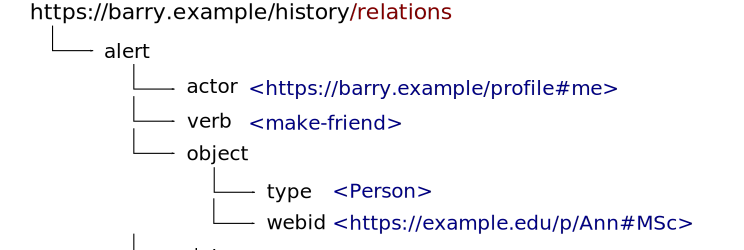
\includegraphics[width=270px]{img/relation_history.pdf}
        \caption{Example of an interaction between Barry and Ann.}
        \label{fig:relation_history}
  \end{center}
\end{figure}

It should be noted that if a user should feel at any time that collecting this information may potentially result in too much exposure of his/her private data, he/she should have the option to disable the Relationship History.

\section{Conclusion}
We believe that based on different contexts and situations, access to resources can be handled differently, especially when coupled with dynamic user relationships. In this chapter we have introduced our third contribution, a social access control service for Web applications, comprised of two distinct sub-services: a \textit{Static Access Control} (SAC) engine and a \textit{Relationship Monitor} engine (RM). Due to existing access control alternatives which handle access control for static documents (Section~\ref{subsec:sem_acl}), our solution is focused on protecting the privacy of Linked Data resources generated by users (e.g. profile data, wall posts, conversations, etc.).\\

The \textit{Static Access Control} engine handles access to user-generated resources, based on predefined privacy policies. The process of permitting/denying access to a resource is quite straightforward, and it involves matching the user performing the request to a list of resources matching the same \textit{context} label. The goal of this process is to finally return a \textit{unique view} of requested resources (e.g. a user's profile), matching to the level of access corresponding to the requesting user.\\

The \textit{Relationship Monitor} engine (RM) relies on metrics such as \textit{context} and \textit{proximity distance} together with a relationship history between the involved actors, in order to either provide notifications for potential privacy issues that may arise when disclosing information, or even to modify existing access control policies for incoming requests (if so configured). The RM applies to two distinct types of actions. First, it is used when assigning context labels when disclosing information, and second for handling a request for a resource.\\

The static access control engine was implemented as a module for MyProfile (Chapter~\ref{ch:implementations}). Unfortunately, we were not able to implement the RM engine for a real application, and therefore we consider this as future work.
